\documentclass[10pt,twocolumn]{article}
\usepackage[margin=0.75in]{geometry}
\usepackage{graphicx}
\usepackage{booktabs}
\usepackage{caption}
\usepackage{subcaption}
\usepackage{hyperref}
\usepackage{amsmath}
\usepackage{xcolor}
\usepackage{float}
\usepackage{enumitem}
\setlist{nosep}

\setlength{\textfloatsep}{6pt plus 2pt minus 2pt}
\setlength{\intextsep}{6pt plus 2pt minus 2pt}
\setlength{\floatsep}{6pt plus 2pt minus 2pt}
\setlength{\abovecaptionskip}{4pt}
\setlength{\belowcaptionskip}{2pt}

\title{COMP 597 -- Energy Profiling of Whisper Fine-Tuning:\\Instrumentation Overhead and Resource Utilization}
\author{Bo Lau\\McGill School of Computer Science\\3480 Rue University, Montreal, QC, H3A 2A7\\bo.lau@mail.mcgill.ca}
\date{}

\begin{document}
\raggedbottom
\maketitle

% ============================================================
\section{Introduction}
% ============================================================

Training workloads are increasingly evaluated not only by accuracy and throughput but by the energy and carbon cost of running them at scale. This project adopts that perspective and studies a fine-tuning scenario derived from the Milabench benchmarking stack~\cite{milabench}, using reported CO$_2$ equivalents from CodeCarbon~\cite{codecarbon} as a primary lens on ``where the carbon goes'' alongside detailed timing and utilization.

Milabench-style setups typically rely on synthetic, in-memory data paths that keep the accelerator busy and abstract away storage. Here we pair that view with a complementary configuration in which fixed-shape Mel spectrograms reside on local SSD and are fed through a conventional PyTorch \texttt{Dataset} and \texttt{DataLoader}. The motivating question was whether moving work off a purely RAM-backed pipeline and onto explicit disk reads would reveal input bottlenecks or qualitatively different energy profiles---for example, if sustained I/O or CPU-side preparation became a first-order concern.

In practice, the behavior we observe is closer to a classical compute-bound regime. Once tensors are resident in the Linux page cache, repeated access from disk is difficult to distinguish from memory-backed serving for this workload, and GPU utilization remains high during steady-state training. The sections that follow detail the Whisper fine-tuning setup, the instrumentation tiers we used to separate measurement overhead from real compute time, and how energy concentrates in the backward pass and GPU power draw despite the two data backends.

% ============================================================
\section{Workload Description}
% ============================================================

\textbf{Model and Task.}
We fine-tune OpenAI's \texttt{whisper-tiny} model~\cite{whisper} for audio classification using the Hugging Face \texttt{WhisperForAudioClassification} architecture. The model is a Transformer-based encoder--decoder with $\sim$39M parameters. We attach a linear classification head and train end-to-end with the AdamW optimizer at a learning rate of $10^{-6}$ on synthetic audio data. No learning rate schedule or weight decay is applied.

\textbf{Data.}
We evaluate two data-loading backends that differ fundamentally in where data resides and how it reaches the GPU:
\begin{itemize}
    \item \textbf{Disk Cache}: The full synthetic dataset (5{,}500 Mel spectrograms) is generated once and saved to a \texttt{.pt} file on local SSD. Every subsequent training run loads this file through a standard PyTorch \texttt{Dataset} and \texttt{DataLoader}, avoiding regeneration. This path exercises the OS storage stack and is subject to Linux page-cache behavior: after the first epoch the file typically resides in RAM-backed page cache, making later reads indistinguishable from memory access.
    \item \textbf{In-Memory (Milabench)}: A small batch of samples is created in RAM and repeated with a configurable repeat factor to reach 16{,}000 logical samples---long enough for a meaningful training run without ever writing or reading a file. Because the data lives entirely in memory, there is no disk I/O and therefore no storage bottleneck to optimize.
\end{itemize}
Both backends produce fixed-shape Mel spectrograms matching Whisper's expected input format (80 frequency bins $\times$ 3000 time steps).

\textbf{Hardware.}
All experiments run on a single SLURM-allocated node (\texttt{gpu-grad-01}) with:
\begin{itemize}
    \item \textbf{GPU}: NVIDIA RTX A5000 (24\,GB GDDR6, 234W TDP)
    \item \textbf{CPU}: AMD EPYC 9554 64-Core (4 cores allocated via SLURM)
    \item \textbf{RAM}: 4\,GB (SLURM job allocation)
    \item \textbf{OS}: Linux 5.15, Python 3.14, PyTorch with CUDA
\end{itemize}

\textbf{Terminology.}
A \emph{step} consists of one forward pass, one backward pass, and one optimizer update on a single batch. Each \emph{phase} (forward, backward, optimizer) is timed individually. Training proceeds for one epoch or until a 5-minute wall-clock limit, whichever comes first.

% ============================================================
\section{Methodology}
% ============================================================

\subsection{Experiment Design}

Each experiment is a 5-minute training run repeated 3 times to account for system variability. We sweep three batch sizes: 32, 64, and 128---the largest power-of-2 that fits in GPU memory and two smaller values. For both data backends, we test 0 and 4 \texttt{DataLoader} workers. With 0 workers, data loading occurs on the main training thread; with 4, background processes prepare batches in parallel.

The number of training steps per run depends on both the dataset size and the time limit:
\begin{itemize}
    \item \textbf{Disk}: one epoch = $\lceil 5500 / \text{batch\_size} \rceil$ steps. At batch~32, this yields 172 steps ($\sim$72\,s with noop), well within 5 minutes.
    \item \textbf{Milabench}: one epoch = $16000 / \text{batch\_size}$ steps. At batch~32, this yields 500 steps ($\sim$211\,s with noop), also within 5 minutes.
\end{itemize}

\subsection{Measurement Setup}

We employ six \emph{trainer stats} modules that instrument the training loop with increasing levels of detail:

\begin{itemize}
    \item \textbf{noop}: All hooks are empty (\texttt{pass}). Baseline for end-to-end wall-clock time with zero instrumentation overhead.
    \item \textbf{simple}: CUDA-synchronized timers before and after each phase. Records forward, backward, and optimizer durations. No resource monitoring or file I/O during training.
    \item \textbf{phase\_times}: Inherits \texttt{simple}'s timing hooks; writes per-step phase durations to a CSV file at the end of training.
    \item \textbf{resource\_util}: Records GPU utilization, GPU power draw, GPU memory (allocated and reserved), CPU utilization, RAM usage, and disk I/O per step via NVML and \texttt{psutil}. CPU utilization is measured with \texttt{psutil.Process().cpu\_percent()}, which reports the \emph{sum} across all cores for the training process (values can exceed 100\%). Also includes phase timing via CUDA sync.
    \item \textbf{codecarbon}: CodeCarbon energy tracking with a 500\,ms power sampling interval, combined with phase timing.
    \item \textbf{codecarbon\_e2e}: CodeCarbon with 86{,}400\,s sampling interval (effectively one sample for the entire run), designed to minimize polling overhead while still capturing total energy.
\end{itemize}

\textbf{GPU Timing Synchronization.}
All timing-capable modules (every module except \texttt{noop}) call \texttt{torch.cuda.synchronize(device)} before and after each phase boundary---8 calls per step total. This ensures that asynchronously dispatched CUDA kernels have completed before timestamps are recorded. Without synchronization, the CPU-side timer would only measure kernel \emph{launch} time, not actual GPU execution time. However, this serializes the GPU pipeline: the CPU cannot enqueue the next operation until the previous one completes, which prevents overlapping data loading with GPU compute.

\textbf{Energy Measurement.}
CodeCarbon samples GPU power via NVML at the configured interval. CPU power is estimated from the processor's TDP rather than measured directly, as RAPL counters were not accessible on the cluster (permission denied). Total energy is reported as the sum of GPU, CPU, and RAM energy. CO$_2$ emissions are computed using CodeCarbon's grid carbon intensity factor for Quebec, Canada.

% ============================================================
\section{Results}
% ============================================================

We organize results into five categories: end-to-end timing, energy consumption, per-phase analysis, system utilization, and instrumentation overhead.

\subsection{End-to-End Execution Time}

Table~\ref{tab:e2e_time} shows the mean training duration for each trainer stats module. With disk loading and \texttt{workers=0}, all instrumented trainers are 30--36\% slower than noop. Crucially, this overhead is nearly identical across \texttt{simple}, \texttt{phase\_times}, and \texttt{resource\_util}---modules that differ substantially in what they measure but all share the same \texttt{torch.cuda.synchronize()} calls. This uniformity demonstrates that the overhead originates from CUDA synchronization, not from the monitoring logic itself.

\begin{table}[H]
\centering
\caption{Mean training duration (seconds), averaged over 3 runs.}
\label{tab:e2e_time}
\small
\begin{tabular}{lrrr}
\toprule
Trainer & B=32 & B=64 & B=128 \\
\midrule
\multicolumn{4}{l}{\textit{Disk, workers=0}} \\
noop            & 72.0 & 71.3 & 70.3 \\
simple          & 95.7 & 94.3 & 92.3 \\
phase\_times    & 96.0 & 93.7 & 94.3 \\
resource\_util  & 98.0 & 95.3 & 94.3 \\
codecarbon      & 98.0 & 93.7 & 91.7 \\
\midrule
\multicolumn{4}{l}{\textit{Disk, workers=4}} \\
noop            & 114.5 & 112.7 & 116.3 \\
simple          & 115.7 & 115.7 & 117.7 \\
resource\_util  & 119.3 & 119.0 & 124.3 \\
codecarbon      & 118.7 & 117.0 & 121.0 \\
\midrule
\multicolumn{4}{l}{\textit{Milabench, workers=0}} \\
noop            & 211.0 & 208.7 & 205.0 \\
simple          & 213.3 & 214.0 & 210.7 \\
resource\_util  & 214.7 & 214.3 & 211.0 \\
codecarbon      & 217.0 & 215.7 & 211.7 \\
\midrule
\multicolumn{4}{l}{\textit{Milabench, workers=4}} \\
noop            & 224.7 & 213.0 & 210.0 \\
simple          & 231.7 & 217.3 & 215.0 \\
resource\_util  & 231.3 & 217.7 & 215.0 \\
codecarbon      & 238.7 & 219.0 & 215.7 \\
\bottomrule
\end{tabular}
\end{table}

When comparing against \texttt{simple} as a baseline (isolating monitoring overhead from sync overhead), resource monitoring adds $<$3\% and CodeCarbon adds 1--6\% on top of the sync cost.

The configuration dependence of overhead is explained by the degree of CPU/GPU overlap lost to synchronization. With \texttt{workers=0} on disk, the main thread can load the next batch \emph{while} the GPU processes the current one---sync destroys this overlap. With \texttt{workers=4}, background processes keep batches ready regardless of main-thread blocking. With Milabench, in-memory data loading is near-instant and does not overlap with GPU execution in any meaningful way, so synchronization has little additional cost to expose.

\subsection{End-to-End Energy Consumption}

Table~\ref{tab:energy} summarizes CodeCarbon energy measurements. Across all configurations, energy breaks down as approximately 65--73\% CPU, 25--34\% GPU, and 2\% RAM. The CPU-dominated breakdown is an artifact of TDP-based estimation; the actual CPU power draw is likely much lower than the reported $\sim$360\,W estimate across all 64 cores, given that only 4 cores are allocated.

\begin{table}[H]
\centering
\caption{Mean energy consumption (kWh) from CodeCarbon, averaged over 3 runs.}
\label{tab:energy}
\small
\begin{tabular}{llrrr}
\toprule
Source & W & B=32 & B=64 & B=128 \\
\midrule
\multicolumn{5}{l}{\textit{Total energy (kWh)}} \\
Disk   & 0 & 0.0142 & 0.0138 & 0.0136 \\
Disk   & 4 & 0.0161 & 0.0160 & 0.0165 \\
Mila.  & 0 & 0.0328 & 0.0330 & 0.0327 \\
Mila.  & 4 & 0.0354 & 0.0334 & 0.0331 \\
\midrule
\multicolumn{5}{l}{\textit{GPU energy only (kWh)}} \\
Disk   & 0 & 0.0042 & 0.0042 & 0.0042 \\
Disk   & 4 & 0.0039 & 0.0040 & 0.0041 \\
Mila.  & 0 & 0.0106 & 0.0110 & 0.0110 \\
Mila.  & 4 & 0.0109 & 0.0109 & 0.0110 \\
\bottomrule
\end{tabular}
\end{table}

Disk experiments consume roughly half the energy of Milabench experiments, proportional to their shorter duration. Energy is relatively stable across batch sizes since runs are time-limited: larger batches complete fewer steps, but each step processes more data. CO$_2$ emissions are very low ($<$0.15\,g per run) due to Quebec's hydroelectric grid.

\subsection{Per-Phase Timing Analysis}

Figure~\ref{fig:phase_bars} shows per-phase mean durations for batch~32. The backward pass dominates at $\sim$290\,ms ($\sim$68\% of step time), followed by forward at $\sim$125\,ms ($\sim$30\%), with the optimizer step negligible at $\sim$2\,ms ($\sim$0.5\%). The backward pass is $\sim$2.3$\times$ slower than the forward pass because it computes gradients for all parameters in addition to traversing the computation graph. The optimizer step is fast because AdamW performs only element-wise updates.

As batch size increases from 32 to 128, both forward and backward durations increase (more data per step), but the optimizer step remains constant since it depends only on the number of parameters, not the batch size. The standard deviation across steps is low ($<$5\,ms for steady-state steps), indicating stable per-step performance after the first warm-up step. Figure~\ref{fig:phase_bars} shows per-phase mean durations and Figure~\ref{fig:phase_violins} shows the per-phase resource distributions.

\subsection{System Utilization}

Figure~\ref{fig:gpu_util} shows GPU utilization across batch sizes. GPU utilization is consistently above 97\% during steady-state training across all batch sizes, confirming that the workload is compute-bound on the RTX~A5000. Step~1 exhibits lower utilization ($\sim$62--90\%) due to CUDA JIT compilation and initial memory allocation, but recovers to near-100\% by step~2.

CPU utilization varies with batch size---$\sim$73\% for batch~32, $\sim$152\% for batch~64, and $\sim$189\% for batch~128 on the 4 allocated cores---reflecting increased data-loading and preprocessing work for larger batches (Figure~\ref{fig:gpu_util_mila}). GPU memory usage scales substantially with batch size: $\sim$6.8\,GB for batch~32, $\sim$12.5\,GB for batch~64, and $\sim$23.9\,GB for batch~128, nearly saturating the 24\,GB A5000 at the largest batch size.

Disk I/O is concentrated at the beginning of training (initial data loading) and is negligible during steady-state steps (Figure~\ref{fig:resources}), confirming that the data fits in the OS page cache after the first pass.

\subsection{Instrumentation Overhead}

Figures~\ref{fig:overhead_w0} and~\ref{fig:overhead} compare the overhead of each trainer stats module relative to noop for \texttt{workers=0} and \texttt{workers=4}, respectively. The overhead hierarchy is:
\begin{enumerate}
    \item \textbf{CUDA synchronization} (shared by all non-noop trainers): 30--36\% with disk/\texttt{workers=0}; 1--7\% with \texttt{workers=4}; 1--5\% with Milabench.
    \item \textbf{Resource monitoring} (NVML, psutil, disk I/O): $<$3\% additional overhead beyond simple timer-based sync.
    \item \textbf{CodeCarbon energy tracking}: 1--6\% additional overhead, with \texttt{codecarbon\_e2e} (sparse sampling) slightly lower than \texttt{codecarbon} (500\,ms polling).
\end{enumerate}

The stark difference between disk/\texttt{workers=0} (30--36\% overhead) and all other configurations (1--7\%) arises from the loss of CPU/GPU pipeline overlap. With \texttt{workers=0}, the main thread loads data asynchronously with GPU execution; CUDA synchronization blocks this overlap, adding $\sim$24\,s to a 72\,s run. With background workers or slower data pipelines, there is less overlap to lose.

% ============================================================
% All figures on a single page
% ============================================================
\begin{figure*}[p]
\centering

\begin{minipage}[t]{0.32\textwidth}
    \centering
    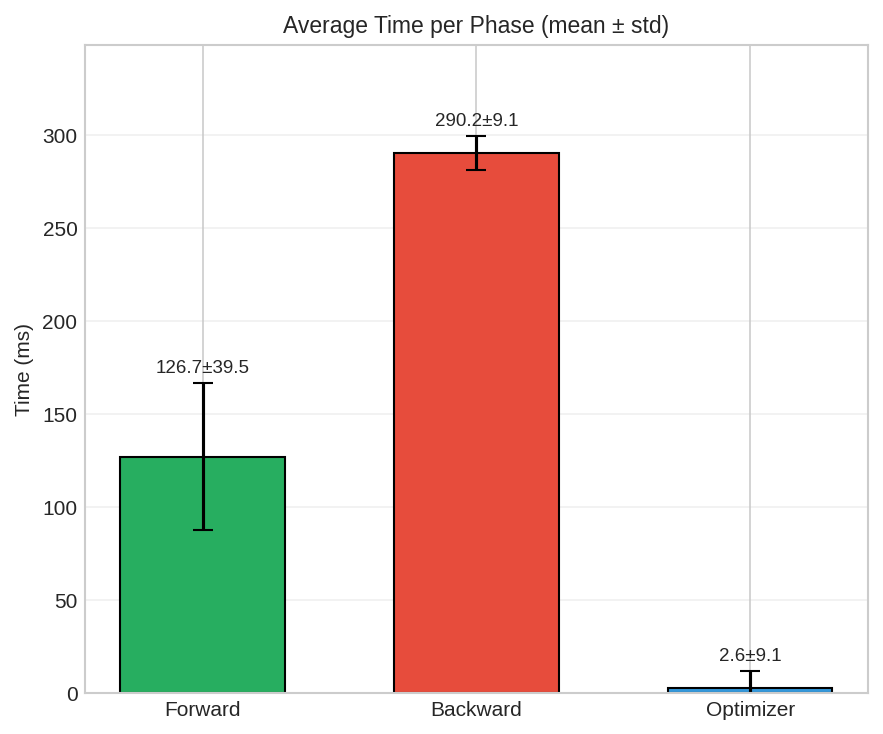
\includegraphics[width=\textwidth]{figures/phase_time_bars_disk_w0_b32.png}
    \captionof{figure}{Per-phase timing (disk, w=0, B=32).}
    \label{fig:phase_bars}
\end{minipage}\hfill
\begin{minipage}[t]{0.32\textwidth}
    \centering
    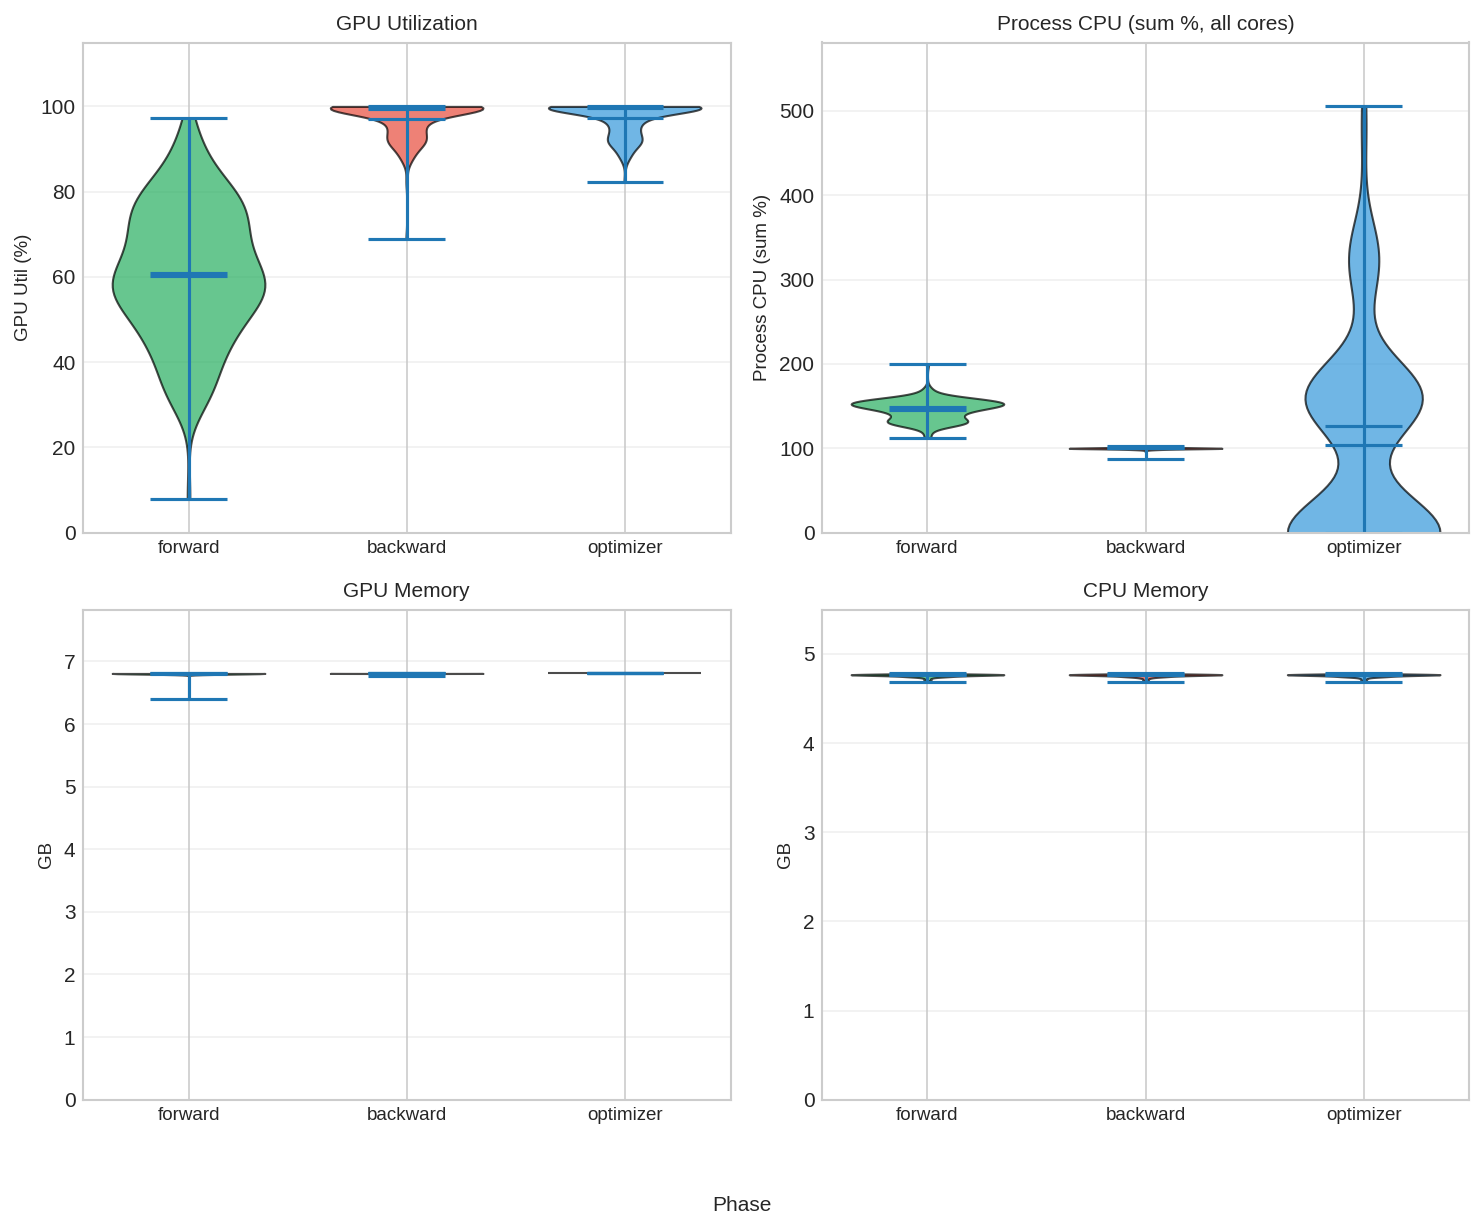
\includegraphics[width=\textwidth]{figures/resource_phases_disk_w0_b32.png}
    \captionof{figure}{Per-phase resource distributions (disk, w=0, B=32).}
    \label{fig:phase_violins}
\end{minipage}\hfill
\begin{minipage}[t]{0.32\textwidth}
    \centering
    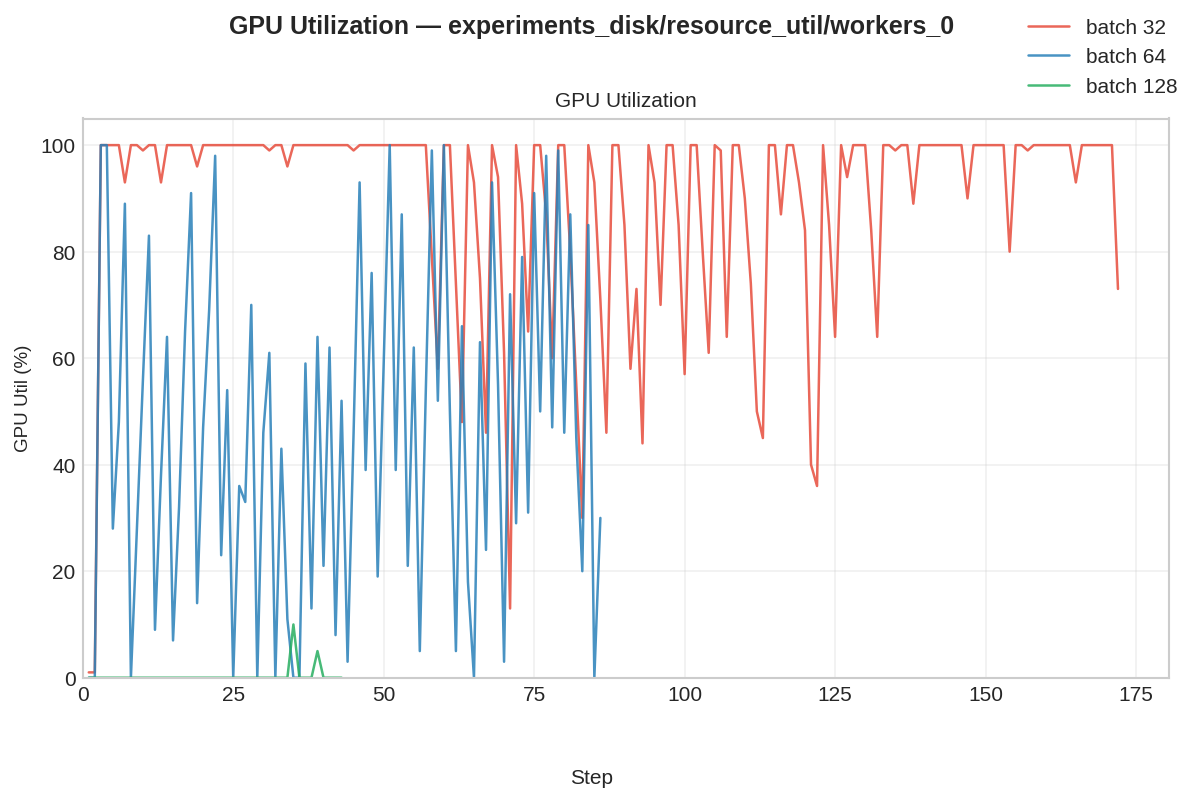
\includegraphics[width=\textwidth]{figures/gpu_util_disk_w0.png}
    \captionof{figure}{GPU utilization across batch sizes (disk, w=0).}
    \label{fig:gpu_util}
\end{minipage}

\vspace{6pt}

\begin{minipage}[t]{0.48\textwidth}
    \centering
    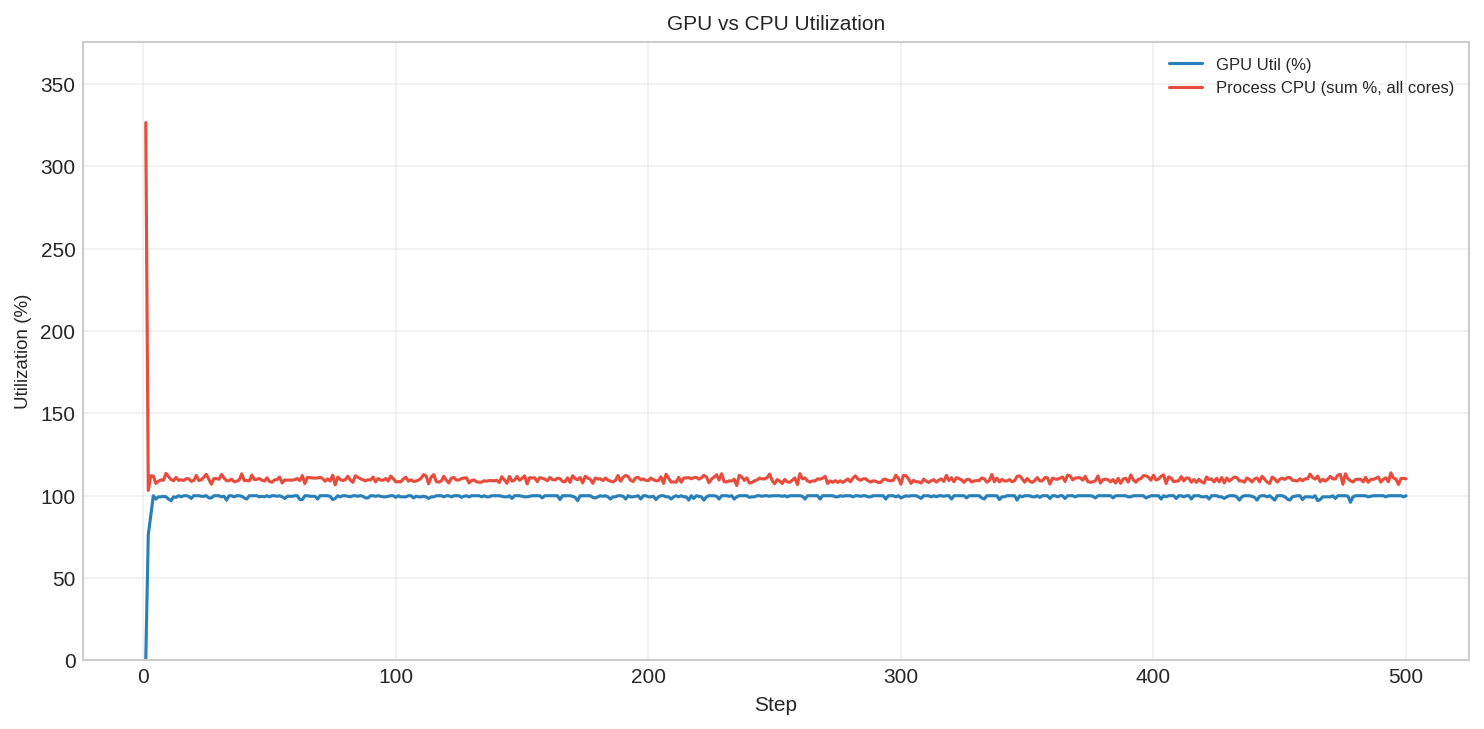
\includegraphics[width=\textwidth]{figures/gpu_cpu_util_mila_w0_b32.png}
    \captionof{figure}{GPU and CPU utilization (Milabench, w=0, B=32).}
    \label{fig:gpu_util_mila}
\end{minipage}\hfill
\begin{minipage}[t]{0.48\textwidth}
    \centering
    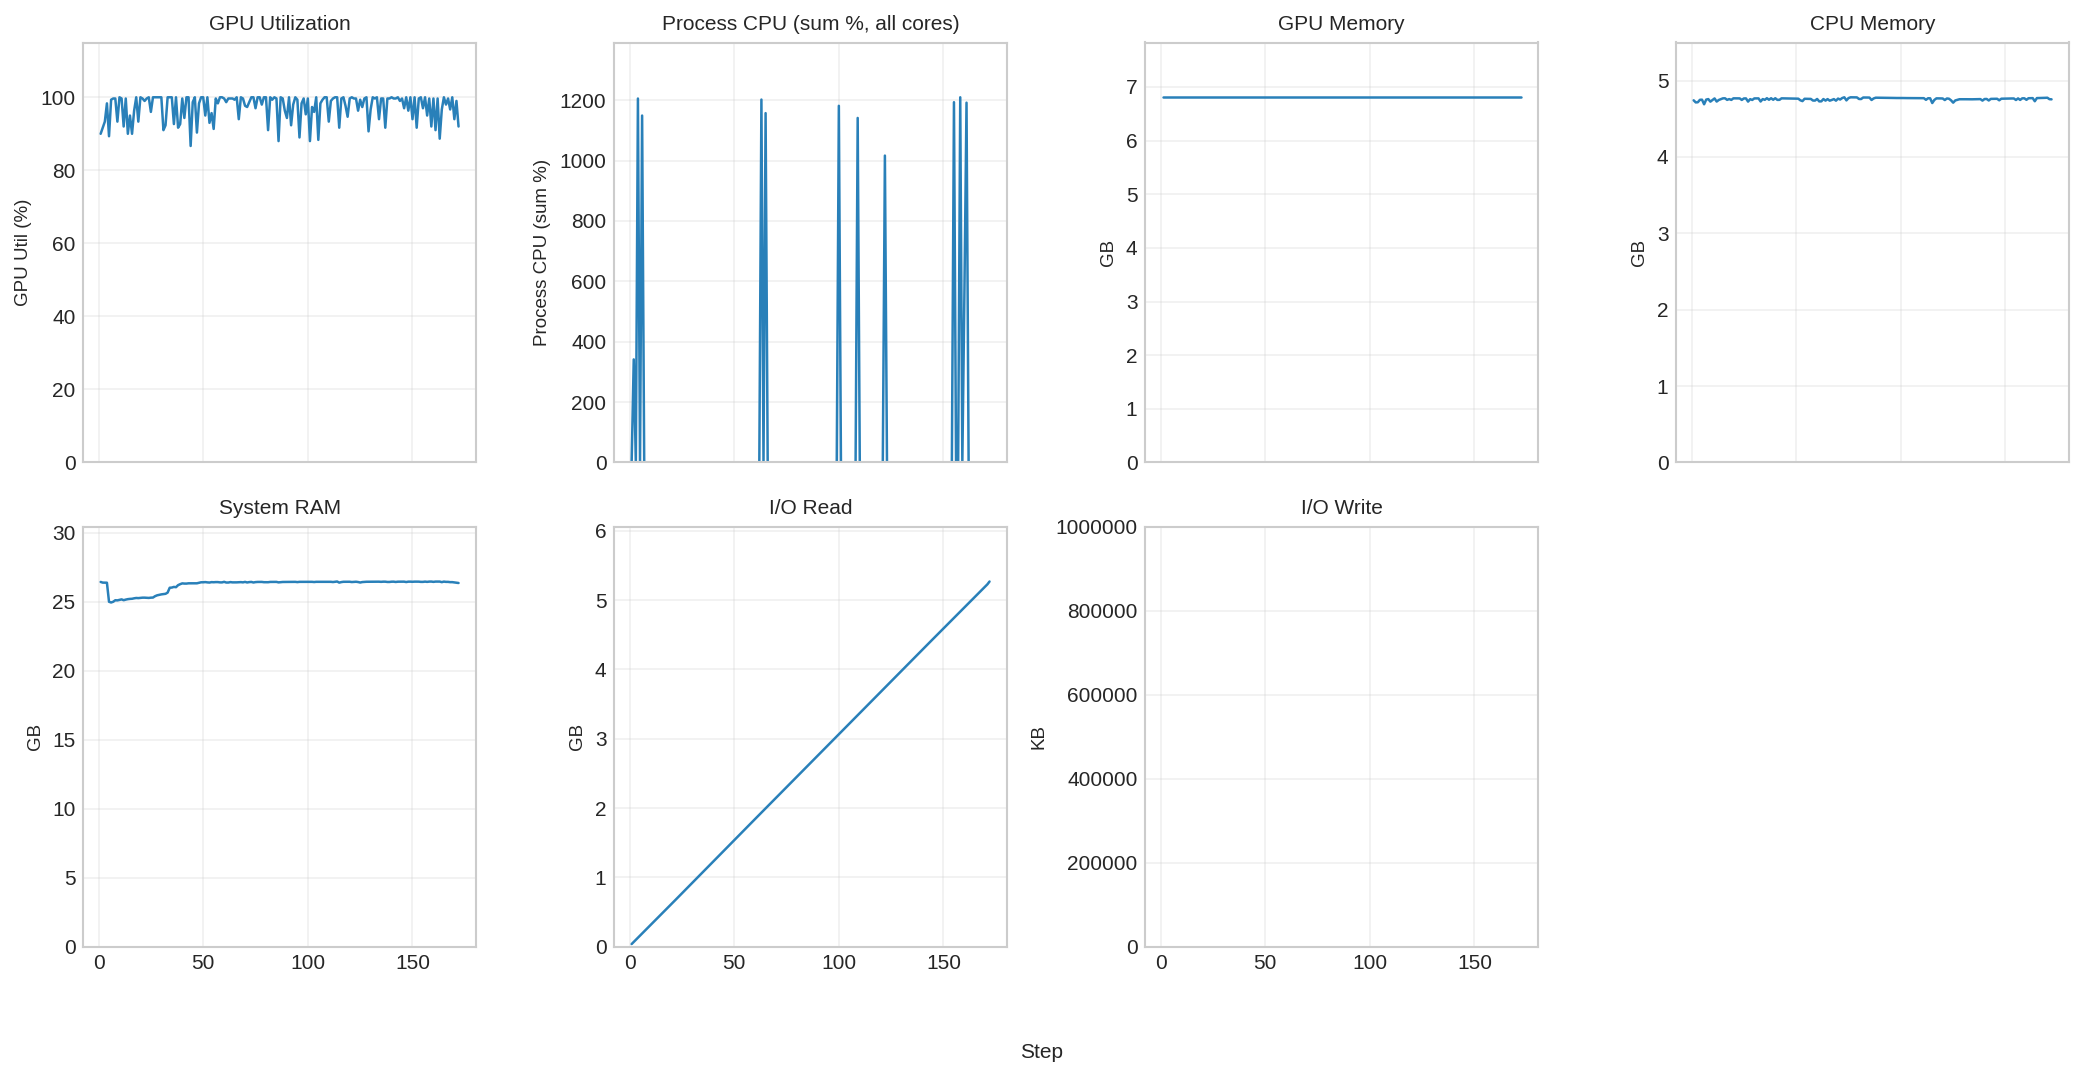
\includegraphics[width=\textwidth]{figures/resources_disk_w0.png}
    \captionof{figure}{Full resource timeline (disk, w=0).}
    \label{fig:resources}
\end{minipage}

\vspace{6pt}

\begin{minipage}[t]{0.48\textwidth}
    \centering
    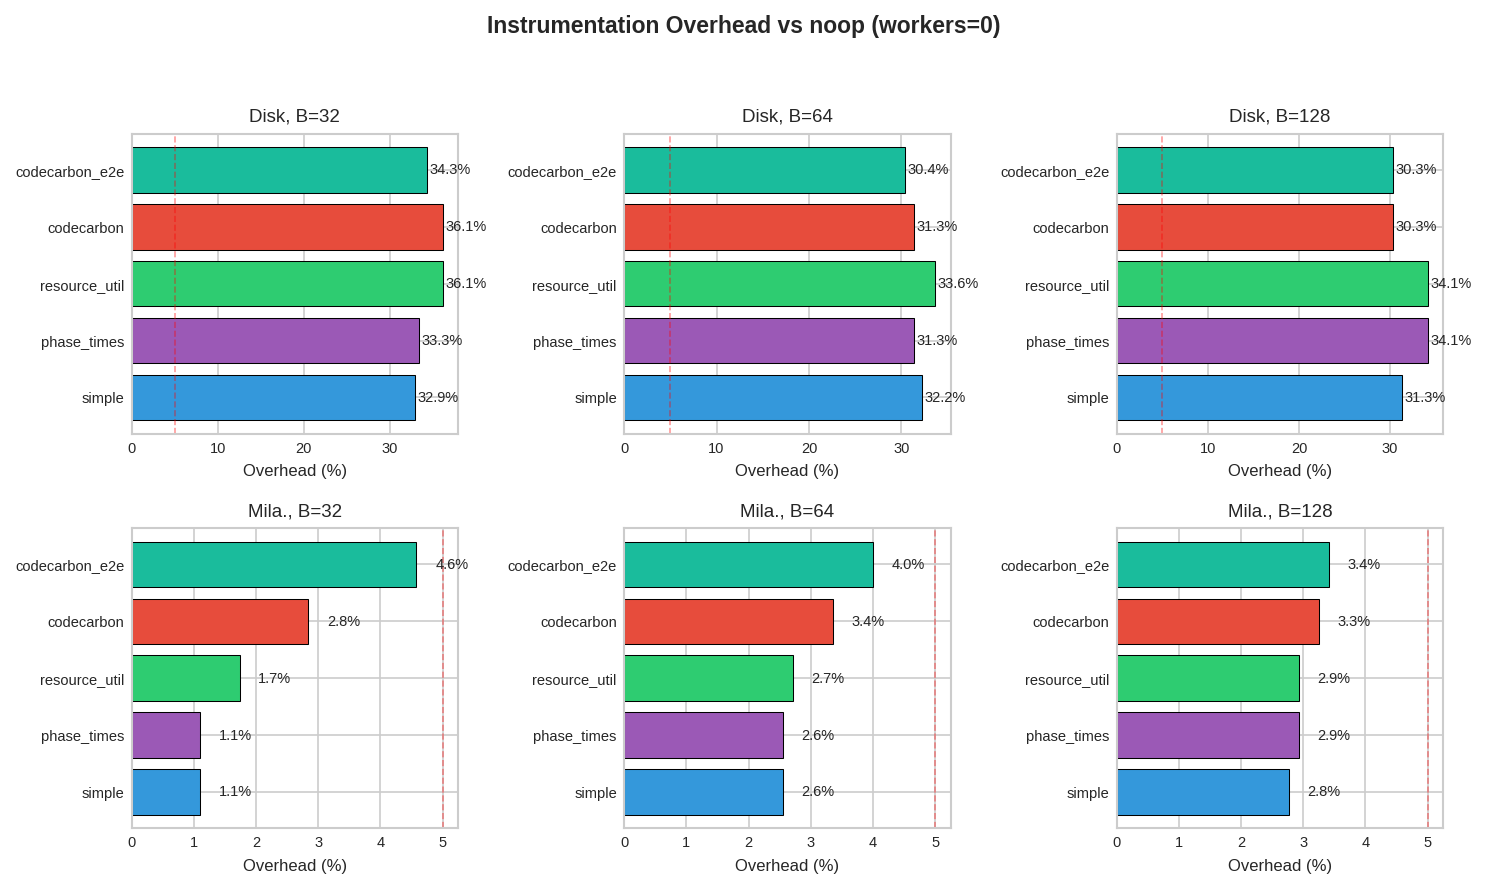
\includegraphics[width=\textwidth]{figures/overhead_vs_noop_w0.png}
    \captionof{figure}{Instrumentation overhead vs.\ noop (workers=0).}
    \label{fig:overhead_w0}
\end{minipage}\hfill
\begin{minipage}[t]{0.48\textwidth}
    \centering
    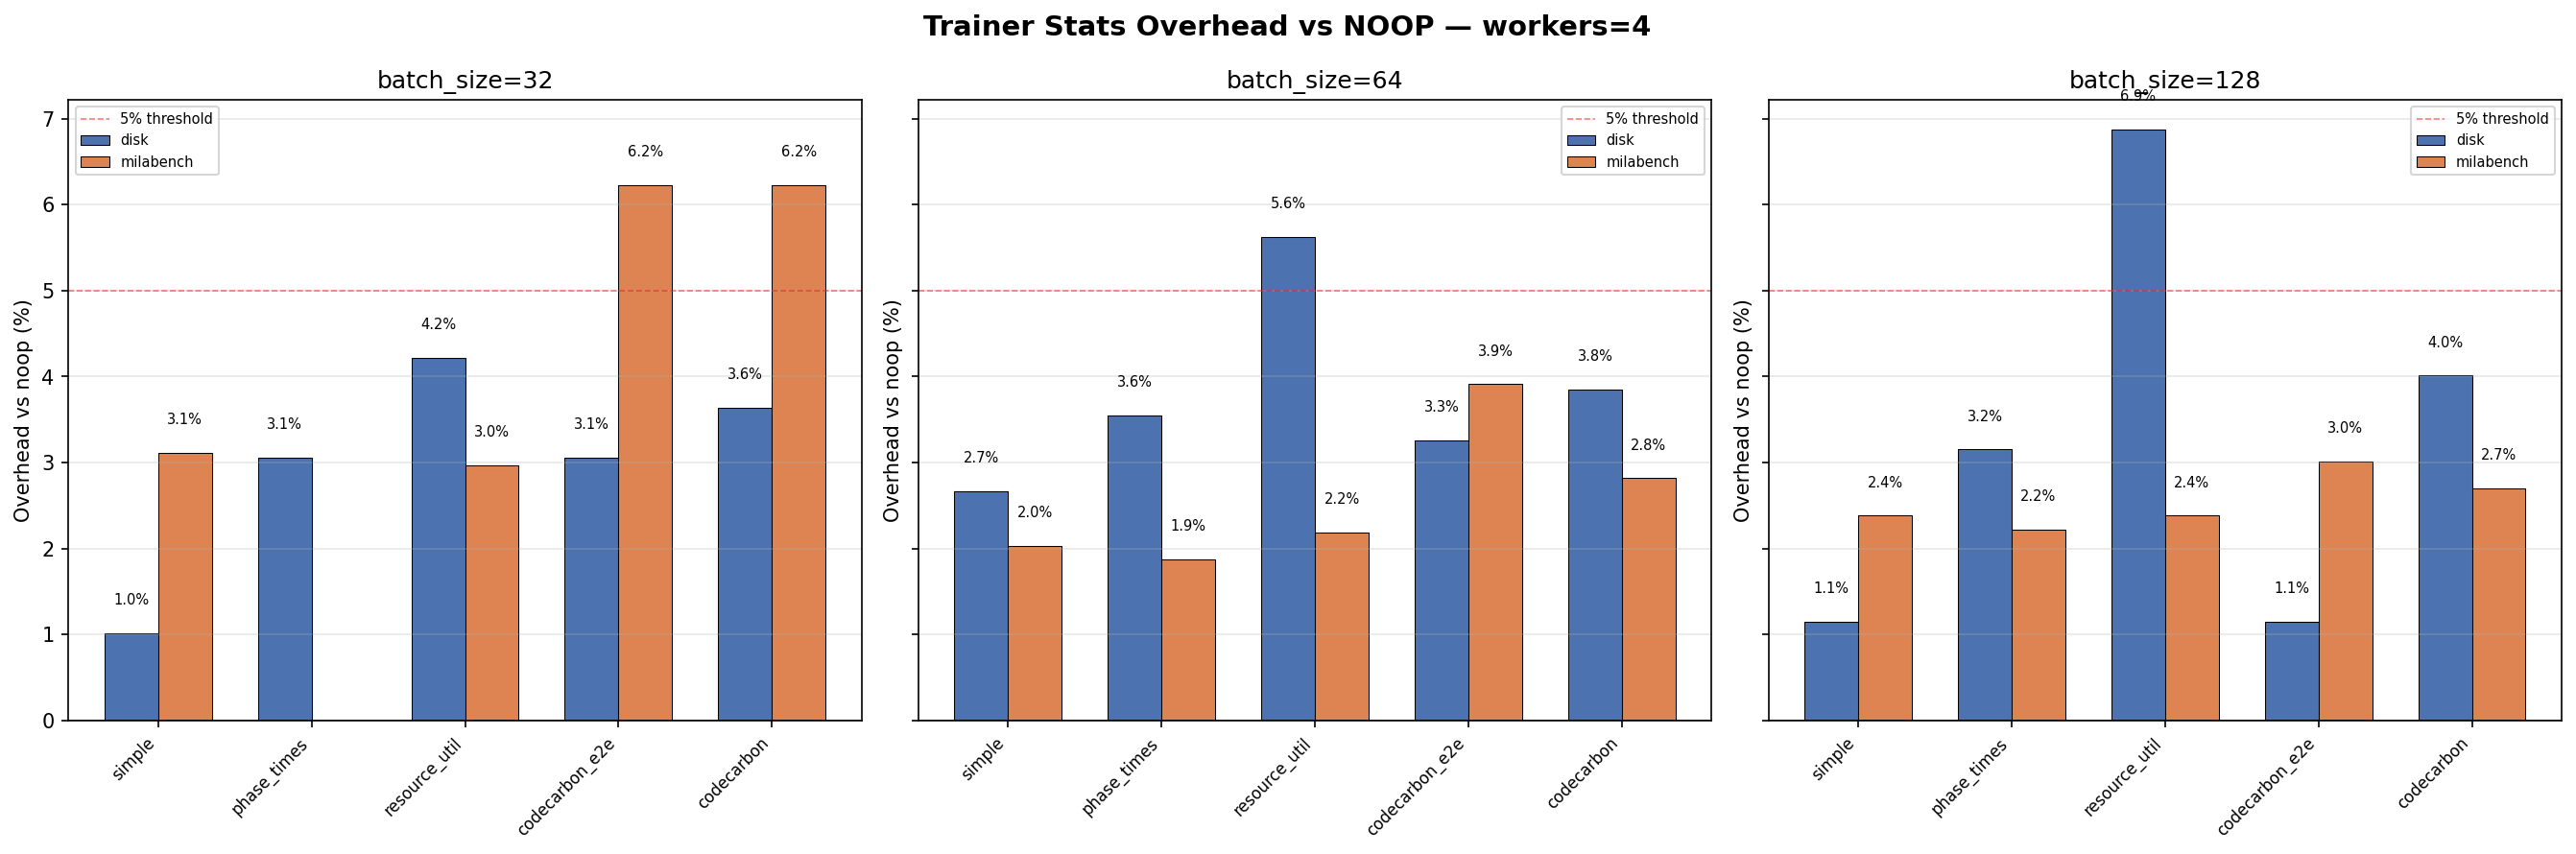
\includegraphics[width=\textwidth]{figures/overhead_vs_noop_w4.png}
    \captionof{figure}{Instrumentation overhead vs.\ noop (workers=4).}
    \label{fig:overhead}
\end{minipage}

\end{figure*}

% ============================================================
\section{Discussion}
% ============================================================

\textbf{Where is energy spent?}
The backward pass dominates compute time at $\sim$68\% of each step, making gradient computation the primary driver of GPU energy consumption. In terms of CodeCarbon's reported total, CPU energy appears to dominate (65--73\%), but this is an artifact of TDP-based estimation: CodeCarbon attributes the full 360\,W TDP of the 64-core EPYC to the process even though only 4 cores are allocated. The actual CPU power draw is likely 20--40\,W, which would make GPU energy the true dominant component at $>$70\% of total.

\textbf{GPU utilization and inefficiency.}
GPU utilization exceeds 97\% during steady-state training for all batch sizes, confirming the workload is compute-bound. The primary source of inefficiency is the first training step, which takes $\sim$2.8$\times$ longer due to CUDA JIT compilation and initial memory allocation. For short runs (5 minutes), this warm-up represents $<$2\% of total time. No significant underutilization periods were observed during steady-state training, suggesting that Whisper fine-tuning on synthetic data saturates the A5000's compute capacity.

\textbf{Batch size, overhead, and practical trade-offs.}
Larger batches yield higher throughput but total energy is roughly constant across batch sizes because runs are time-limited (Table~\ref{tab:energy}). The dominant measurement overhead is \texttt{torch.cuda.synchronize()}, required for accurate GPU phase timing but not a tool limitation---it is a fundamental property of CUDA's asynchronous model. With background workers (\texttt{workers=4}), overhead is $<$7\% across all configurations, acceptable for profiling. For production training the \texttt{noop} module provides zero overhead.

\textbf{Data loading: disk cache vs.\ in-memory.}
The disk cache backend serializes the dataset to a \texttt{.pt} file on SSD; after the first access the Linux page cache serves it from RAM, so steady-state disk I/O is effectively zero (Figure~\ref{fig:resources}). The in-memory Milabench backend keeps all data in RAM by construction---no file is ever read or written---eliminating any storage bottleneck and keeping GPU utilization near 100\%. However, this in-memory design is not representative of production workloads where datasets (raw audio, images, large corpora) exceed RAM and must be streamed from disk or networked storage, making I/O a potential first-order bottleneck. In our experiments both backends produce nearly identical GPU utilization ($>$97\%) because the synthetic dataset fits in page cache, but workloads with larger datasets would likely show a different picture.

\textbf{Limitations.}
(1)~CPU energy is TDP-estimated, not measured via RAPL, so the reported CPU/GPU energy split is unreliable. (2)~Training duration is parsed from tqdm with integer-second precision; sub-second accuracy would require additional high-resolution timers. (3)~All experiments use synthetic data; real audio datasets with variable-length inputs and I/O-bound loading patterns may exhibit different utilization profiles. (4)~We profile a single GPU; multi-GPU training would introduce communication overhead not captured here.

\begin{thebibliography}{9}
\bibitem{milabench} Milabench contributors, ``Milabench,'' GitHub repository, \url{https://github.com/milabench/milabench}.
\bibitem{codecarbon} CodeCarbon contributors, ``CodeCarbon: Track emissions from computing,'' \url{https://github.com/mlco2/codecarbon}.
\bibitem{whisper} A.~Radford et al., ``Robust Speech Recognition via Large-Scale Weak Supervision,'' \textit{Proc. ICML}, 2023.
\end{thebibliography}

\end{document}
